\documentclass[12pt]{scrartcl}

\usepackage{hyperref}
\usepackage{tabularx}
\usepackage{pdflscape}
\usepackage{caption}
\usepackage{verbatim}
\usepackage{multirow}
\usepackage{ltablex}
\usepackage{enumitem}
\usepackage{amssymb}
\usepackage{graphicx}
\usepackage{float}
\usepackage[parfill]{parskip}

\hypersetup{
	pdftitle={Basic Sailng 1 - Course Material},
	pdfauthor={Chaitanya Chowgule},
	colorlinks=true,
	linkcolor=blue
}

\setcounter{tocdepth}{2}

\title{Basic Sailing 1}
\subtitle{Course Material}
\date{}

\newlist{test}{itemize}{1}
\setlist[test]{label=$\square$}

\graphicspath{{/media/interchange/WD/Sailing/PNGs/}}

\makeatletter
\renewcommand{\@seccntformat}[1]{}
\makeatother

\captionsetup[figure]{labelformat=empty}

\begin{document}

\maketitle

\thispagestyle{empty}

\tableofcontents

\newpage

\section{Outline} \label{sec:outline}

This course aims to introduce complete novices to the most fundamental sailing techniques such as steering, sail trim, tacks, and gybes. It is perhaps the most important as without these fundamentals future courses will be much harder to teach. The aim is to build a strong base and ensure that new sailors do not develop bad habits that may make it harder for them to sail in more challenging conditions. The course will be conducted on a reach-to-reach course about 8 boat lengths long.

\subsection{Course Goals} \label{subsec:course goals}

Participants should leave the course having mastered:

\label{list:goals}
\begin{enumerate}
	\item Basics of steering
	\item Identifying points of sail
	\item Identifying major roles on a Seabird
	\item Steering to a course or to a sail setting
	\item Trimming to a course or a point of sail
	\item Controlled stops and starts
	\item Basic tack without getting stuck in irons
	\item Basic gybe while maintaining control of direction and sail
\end{enumerate}

\subsection{Course Requirements} \label{subsec:course requirements}

\label{tab:requirements}
\begin{tabular}{rl}
	Conditions: & Light Day \\
	Grade: & None \\
\end{tabular}

\newpage

\section{Schedule} \label{sec:schedule}

\label{tab:schedule}
\begin{tabularx}{\textwidth}{|X|X|}
	\hline
	\textbf{Time} & \textbf{Activity} \\
	\hline
	25 mins. & Setup for course before participants arrive. Sign out all materials needed for the course and make sure they are in working order. Load materials needed on the water on the powerboat and confirm it is fuelled. Set the training course. \\
	\hline
	30 mins. & Briefing: \\
	& Get to know the participants. Names, when the did the previous courses, etc. \\
	& Refresh skills and info from previous courses relevant to this course. \\
	& List all skills to be covered today and go over the sailing area and the course. \\
	& Go through skills individually paying careful attention to common mistakes and how to correct them. \\
	& Explain the test and its criteria for passing. \\
	\hline
	10 mins. & Head out to the boat, rig up and sail to the training course. \\
	\hline
	2 hrs. & Go through the skills. Have them rotate roles every 4 completed circuits. \\
	\hline
	10 mins. per test taker & Conduct the test for participants whom you feel are ready. \\
	\hline
	15 mins. & Return to the mooring. Have the Tindle pick up the training course. \\
	\hline
	30 mins. & Debriefing: \\
	& Recap all skills covered on the water \\
	& Point out common mistakes and single out those who corrected them successfully. Explain how they did so. \\
	\hline
	10 mins. & Clear the powerboat and briefing area. Return all items and sign them back in. \\
	\hline
\end{tabularx}

Total time: 4 hrs. 10 mins. to 4 hrs. 40 mins.

\newpage

\section{Syllabus} \label{sec:syllabus}

\subsection{Setup} \label{subsec:setup}

{\small \textit{25 mins.}}

Before the participants arrive check that the weather conditions acceptable for the course and decide on the sailing area for the day.

Sign out the following:

\label{list:materials}
\begin{itemize}
	\item Whiteboard, markers and figures
	\item 2 marks with anchors and anchor lines
	\item Wind indicator
\end{itemize}

Load the marks on to the powerboat and ensure there is enough fuel for the day.

Go out with the Tindle and set the training course.

Set up the whiteboard for the briefing.

\subsection{Briefing} \label{subsec:briefing}

{\small \textit{30 mins.}}

Gather the participants in front of the whiteboard, take down their names, and confirm that they have completed the relevant prerequisite courses. If someone has mistakenly come to a course they are not yet qualified to attend inform them which course they should be attending and if possible help them schedule a time to complete it.

On the whiteboard illustrate where on the river the course will be taking place, show the orientation of the marks in relation to some landmark, and if possible point it out from the briefing location.

Start by refreshing material from previous courses. Go over finding the wind direction, estimating wind speed, parts of the boat and their names, leaving and coming to the mooring, etc., briefly.

List out all the skills that will be covered during the course, very briefly expanding on each one.

Go down the list of skills explaining the salient points of each one:

\subsubsection{Basics of steering} \label{subsubsection:basics of steering}

Explain the basics of luffing up and bearing away. Emphasise the need to make small movements for course corrections and large ones for tacks and gybes. Explain the need to make sure the tiller is centred to maintain a straight course.

\subsubsection{Identifying points of sail} \label{subsubsec:points of sail}

Using the points of sail diagram, illustrate the various points of sail and their names. Describe in general how the sails are loosened as the boat is steered away from the wind. Go over the no go zone and how to sail upwind by going from tack to tack. Using the diagram explain how tacks take the bow through the wind causing the sail to change sides and gybes take the stern through the wind with the same result. Then add in an illustration of the days course showing how the marks will create a reach-to-reach course. Point out where the boat will have to tack or gybe to round the course.

\label{fig:points of sail}
\begin{figure}[H]
	\centering
	
\includegraphics[scale=0.5]{Points}
	\caption{Points of Sail Diagram}
\end{figure}

\subsubsection{Identifying major roles on a Seabird} \label{subsubsec:identifying major roles}

Transition to the roles on the Seabird and how the changes in course will be handled by each. Start with the helm, the main sheet trimmer, the person responsible for the runners and centreboard and finally the jib trimmer.

Draw and illustration of the Seabird from a top view and mark where each person should be sitting. Detail how they should cross the boat during a tack or a gybe.

\label{fig:seating}
\begin{figure}[H]
	\centering
	\includegraphics[scale=0.75]{Seating}
	\caption{Seating Positions}
\end{figure}

\subsubsection{Steering to a course or sail setting \& trimming to a course or a point of sail} \label{subsubsec:steering and trimming}

Introduce the 2 major modes of steering. Explain that when steering to a course the helm maintains a steady heading while the trimmers adjust the sails to the course while when steering to a point of sail the trimmers set the sails and the helm must maintain boat speed by adjusting the heading.

\subsubsection{Controlled starts and stops} \label{subsubsec:controlled starts and stops}

Paying close attention to the difference between being in irons and being in a controlled stop, go over the procedure for coming to a stop, maintaining a stationary position, and building boat speed to come out of a stop.

\subsubsection{Basic tacks without getting stuck in iron} \label{subsubsec:basic tacks}

Go over the following tacking drill asking the participants to say the steps out loud:

\label{tab:tacking drill}
\begin{tabularx}{420pt}{lX}
	\centering
	\textbf{1.} & \textbf{Helm:} Look around you to make sure it is safe to tack and to identify a stationary point that the boat should be pointing at when the tack is completed. \\
	& \\
	\textbf{2.} & \textbf{Helm:} Call "ready to tack" and wait for a response from each person on the boat. \\
	& \textbf{Crew:} Call "ready" when you are ready to tack. \\
	& \\
	\textbf{3.} & \textbf{Helm:} Push the tiller away from you as far as it will go. \\
	& \textbf{Runners:} Uncleat the current leeward, soon to be windward, runner and prepare to tighten the current leeward, soon to be windward runner. \\
	& \textbf{Jibsheet trimmer:} Uncleat the current jibsheet while holding the tension. Prepare to tighten the lazy jibsheet through the tack. \\
	& \\
	\textbf{4.} & \textbf{Helm:} Holding the tiller at the extreme position, look forward to see when the boat is pointing at the stationary point indicating the end of the tack. \\
	& \textbf{Mainsheet trimmer:} As the boom crosses the boat guide the slack mainsheet over, then cross to the other side of the boat. \\
	& \textbf{Runners:} Once the boom has crossed the boat, cross to the other side of the boat and tighten the new windward runner. \\
	& \textbf{Jibsheet trimmer:} Once the jib is fully backed, hold it for a few seconds before releasing the old jibsheet, crossing to the other side of the boat, and tightening the new jibsheet. \\
	& \\
	\textbf{5.} & \textbf{Helm:} Once the boat is pointing at the stationary point, centre the tiller and cross to the other side of the boat. \\
\end{tabularx}

Stress the need to back the jib and keep the tiller at the extreme till the boat completes the tack to avoid ending up in irons, and to cross to the other side of the boat facing forward so as to be able to see where the boat is going through the tack.

\subsubsection{Basic gybes while maintaining control of direction and sail} \label{subsubsec:basic gybe}

Go over the following gybing drill asking the participants to say the steps out loud:

\label{tab:gybing drill}
\begin{tabularx}{420pt}{lX}
	\centering
	\textbf{1.} & \textbf{Helm:} Look around you to make sure it is safe to gybe and to identify a stationary point that the boat should be pointing at when the gybe is completed. \\
	& \\
	\textbf{2.} & \textbf{Helm:} Call "ready to gybe" and wait for a response from each person on the boat. \\
	& \textbf{Crew:} Call "ready" when you are ready to gybe. \\
	& \\
	\textbf{3.} & \textbf{Helm:} Pull the tiller toward you about halfway as far as it will go. \\
	& \textbf{Runners:} Uncleat the current leeward, soon to be windward, runner and prepare to tighten the current leeward, soon to be windward runner. \\
	& \textbf{Jibsheet trimmer:} Uncleat the current jibsheet while holding the tension. Prepare to tighten the lazy jibsheet through the tack. \\
	& \\
	\textbf{4.} & \textbf{Helm:} Holding the tiller at its current position, look forward to see when the boat is pointing at the stationary point indicating the end of the gybe. \\
	& \textbf{Mainsheet trimmer:} Pull the mainsheet in from above the block holding all 3 lines, guide the boom over to the other side of the boat and slowly release the mainsheet on the new side. Cross to the other side of the boat. \\
	& \textbf{Runners:} Once the boom has crossed the boat, cross to the other side of the boat and tighten the new windward runner. \\
	& \textbf{Jibsheet trimmer:} Once the jib starts to back, release the old jibsheet, cross to the other side of the boat, and tighten the new jibsheet. \\
	& \\
	\textbf{5.} & \textbf{Helm:} Once the boat is pointing at the stationary point, centre the tiller and cross to the other side of the boat. \\
\end{tabularx}

Remind participants to focus on controlling the main sail as it crosses the boat and stopping the turn as soon as the new course is reached.

\subsubsection{Explain the test and its criteria for passing} \label{subsubsec:test}

Explain to participants that in order to pass, each of them must perform the following at the helm:

\begin{itemize}
	\item Perform 2 tacks from port to starboard and 2 tacks from starboard to port, leaving them with sufficient boat speed, and without getting stuck in irons.
	\item Perform 2 gybes from port to starboard and 2 gybes from starboard to port, maintaining control of the boat by stopping the gybe at the appropriate heading, and having their mainsheet trimmer correctly guide the boom across the boat.
	\item Complete the reach-to-reach course 4 times, leaving the marks to port twice and to starboard twice. Participants must pass each mark within 2 boat lengths of them.
\end{itemize}

\label{fig:test course}
\begin{figure}[H]
	\centering
	
\includegraphics[scale=0.75]{BS1_Course}
	\caption{Test Course}
\end{figure}

\subsection{On the Water} \label{subsec:on the water}

{\small \textit{2 hrs. 10 mins.}}

Begin by performing each of the skills yourself, going around the course twice (once leaving the marks to port and once to starboard).

Have the participants perform the skills, going around the course 4 times (twice leaving the marks to port and twice to starboard), then switch roles by having the helm move to the mainsheet, the mainsheet trimmer to the runners, the runners to the jib, and the jib trimmer to the helm.

Do this cycle till each participant has done each of the roles.

\subsection{Take the Test} \label{subsec:take the test}

{\small \textit{10 mins. per test taker}}

For those whom you feel are ready you can take the test immediately.

For those whom you feel would benefit from practice, ask them to come back at their convenience, informing the tindles when they book the boat that they would like to practice the Basic Sailing 1 test. The tindles will then lay a training course for them to practice the skills taught in this course. Once they have done so a couple of times they can schedule just the test with a qualified member.

\subsection{Debrief} \label{subsec: Debrief}

{\small \textit{45 mins.}}

Once the on water training and test is completed, ask the Tindle to pick up the training course while you head back to the mooring with the participants and unrig the boat.

Once back on shore begin the debrief.

Recap all skills covered that day. Point out common mistakes and remind participants when they made them. In particular remind participants of times when someone made a common mistake and corrected it themselves. Go over any questions participants might have.

For those who need practice before taking the test, explain how they can schedule it. For those who have passed the Basic Sailing 1 test, update their statuses and go over their next steps.

\subsection{Packing Up} \label{subsec:packing up}

{\small \textit{10 mins.}}

Clear all the equipment from the powerboat. Rinse down the marks, anchor lines, and anchors. Clean the whiteboard. Sign all items checked out back into the store and sign for the fuel used that day.

\newpage
\thispagestyle{empty}
\begin{Large}

	\section{Basic Sailing 1 Test} \label{sec:test}

	\begin{tabular}{r}
		Participant's Name:\\
		Instructor's Name:\\
	\end{tabular}

	\vspace{3cm}

	\begin{test}
	\item Performed 2 tacks from port to starboard and 2 from starboard to port.
	\item Performed 2 gybes from port to starboard and 2 from starboard to port.
	\item Completed training course 4 times, twice leaving marks on port and twice leaving marks on starboard.
	\end{test}

	\vspace{3cm}

	Comments:

\end{Large}

\end{document}
